\documentclass{ximera}

%% Where to find images
\graphicspath{  %% When looking for images,
{./}            %% look first at your level,
{./basics/}     %% then in this folder,
}    

\title{Setup a GitHub repository}

\author{Bart Snapp}

\begin{document}
\begin{abstract}
  How to set up your Ximera files in GitHub.
\end{abstract}
\maketitle

\textbf{All Ximera files must be hosted in a Git repository.} You have two
choices when creating new content:
\begin{itemize}
  \item If you are \textbf{starting fresh}, fork the \texttt{ximeraFirstSteps}
        repository.
  \item If you are starting with an \textbf{existing a Git repository}, that is not currently deploying Ximera content, move files
        from \texttt{ximeraFirstSteps} to this repository.
\end{itemize}
We'll address each of these methods in-turn below.
% See the \link[git manual]{http://git-scm.com} for more information about the
% \verb!clone! and \verb!fork! commands.

\section{Starting fresh and forking \texttt{ximeraFirstSteps}}

Forking a repository is well-documented on
\link[GitHub]{https://docs.github.com/en/pull-requests/collaborating-with-pull-requests/working-with-forks/fork-a-repo}.
Basically, you login to GitHub, return to this page, and at the top right there
will be an option to `Fork' this repository. Fork the repo. Accept all
defaults, though you might want to change the name of the repository at this
point. When done, it will take you to
your copy of this repository on GitHub. It will be located someplace like:
\begin{center}
  \texttt{https://github.com/YOUR-GIT-USER-NAME/your-new-repo-name}
\end{center}
Once the repository is forked, clone the forked repository (the one in your
user-space) onto your computer. \textbf{If you are using Windows, be sure to
  clone through WSL.}
After the repository is on your computer, delete all files \textbf{except:}
\begin{itemize}
  \item \texttt{.gitignore}
  \item \texttt{DOTximeraserve}
  \item \texttt{.vscode}
  \item \texttt{scripts}
  \item \texttt{.git}
  \item \texttt{README.md}
  \item \texttt{NOT-THE-LICENSE.md}
\end{itemize}
You must keep the files above.	Commit your changes to GitHub and view your
repository online via a web browser to ensure that the files were deleted.

\section{Starting from an existing GitHub repository}

Starting from an existing GitHub repository, you will need to \textbf{copy}
\begin{itemize}
  \item \texttt{gitignore}
  \item \texttt{.vscode}
  \item \texttt{scripts}
  \item \texttt{README.md}
  \item \texttt{NOT-THE-LICENSE.md}
\end{itemize}
into your repository. If you already have a \verb|.gitignore| file, we suggest
you replace yours with ours. Commit your changes to GitHub and view your
repository online via a web browser to ensure that the files were added.

DISCUSSION ABOUT LICENSE

EDIT/MOVE TO THE REPO .ximerserve



\section{Setting up a Ximera \texttt{xourse}}

Ximera documents can be ``taped'' together using the \texttt{xourse} document
class.
A \verb|xourse| file is basically a list of other \verb|ximera| files and even
other \verb|xourse| files.
The \verb|xourse| file for \textit{First Steps in Ximera} can be found here:
\begin{center}

  \url{https://github.com/ximeraProject/ximeraFirstSteps/aFirstStepInXimera.tex}
\end{center}

This gets complicated because we insist that Ximera documents must compiled not
only when in a \verb|xourse| file, but also individually.
\begin{center}
  \scalebox{.7}{
    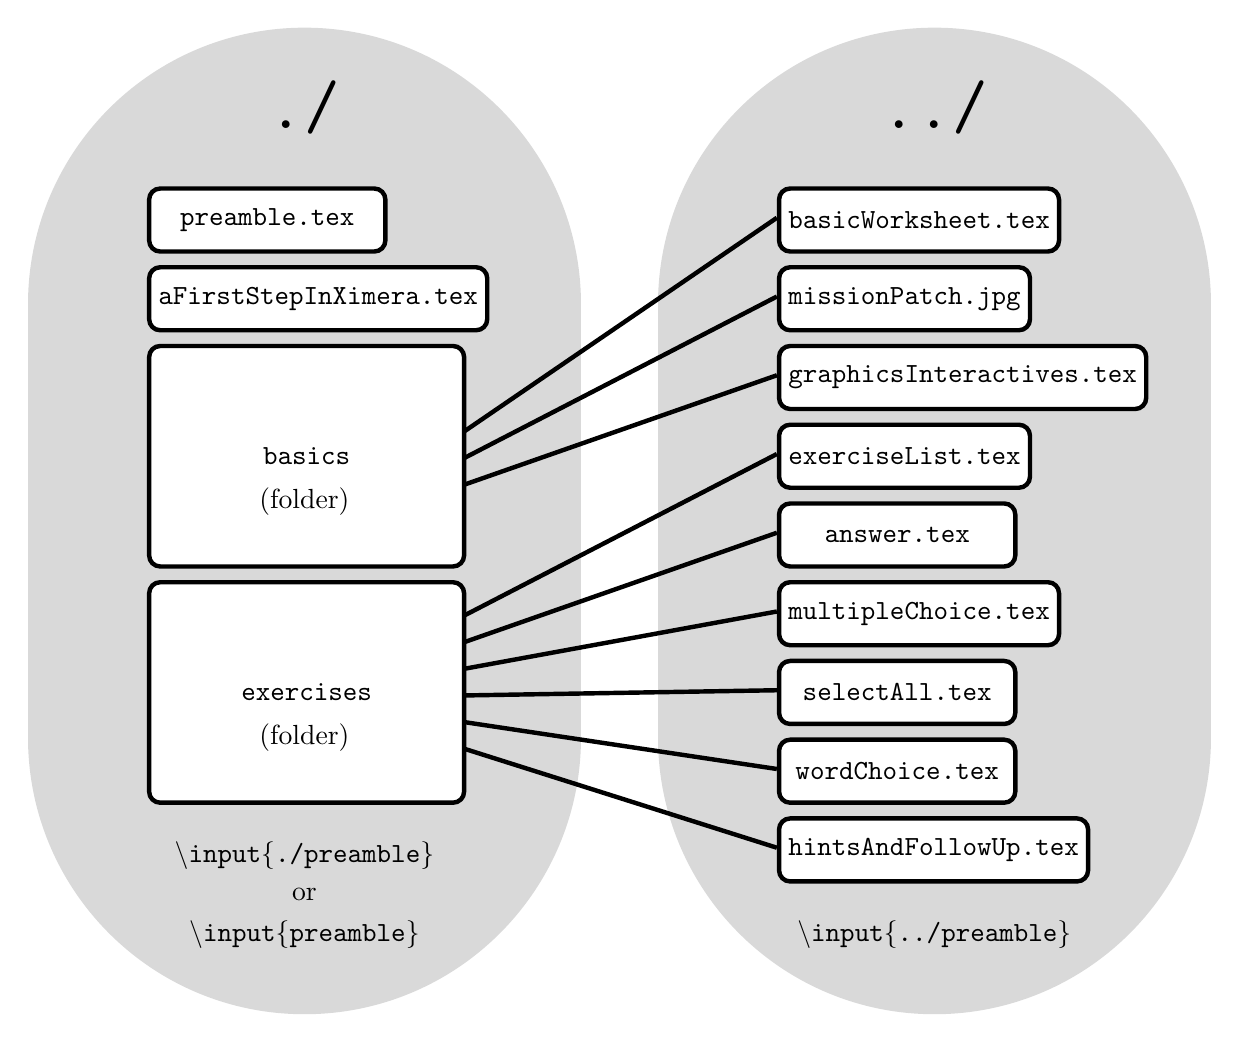
\begin{tikzpicture}
      % Define styles for nodes
      \tikzstyle{document} = [anchor=north west,draw, rounded corners, rectangle,
      minimum width=3cm,fill=white, minimum height=.8cm, ultra
      thick,font=\ttfamily]
      \tikzstyle{folder} = [anchor=north west,draw, rectangle, rounded corners,
      minimum width=4cm,fill=white, minimum height=2.8cm, ultra
      thick,font=\ttfamily]

      % Thick grey lines
      \draw[line width=200pt,white!85!black,line cap=round] (2,1.5) -- (2,-4);
      \draw[line width=200pt,white!85!black,line cap=round] (10,1.5) -- (10,-4);

      % Connections
      \draw[ultra thick] (2,-1.5) -- (8,2.6);
      \draw[ultra thick] (2,-1.5) -- (8,1.6);
      \draw[ultra thick] (2,-1.5) -- (8,.6);

      \draw[ultra thick] (2,-3.5) -- (8,-.4);
      \draw[ultra thick] (2,-3.5) -- (8,-1.4);
      \draw[ultra thick] (2,-3.5) -- (8,-2.4);
      \draw[ultra thick] (2,-3.5) -- (8,-3.4);
      \draw[ultra thick] (2,-3.5) -- (8,-4.4);
      \draw[ultra thick] (2,-3.5) -- (8,-5.4);

      % Symbols at top
      \node at (2,4) {\Huge \tt ./};
      \node at (10,4) {\Huge \tt ../};

      % Define the folders at top level
      \node[document] at (0,3) {preamble.tex};
      \node[document] at (0,2) {aFirstStepInXimera.tex};
      \node[folder] at (0,1) {basics};
      \node[] at (2,-1) {(folder)};
      \node[folder] at (0,-2) {exercises};
      \node[] at (2,-4) {(folder)};


      % Define the documents in the basics folder
      \node[document] at (8,3) {basicWorksheet.tex};
      \node[document] at (8,2) {missionPatch.jpg};
      \node[document] at (8,1) {graphicsInteractives.tex};

      % Define the documents in the exercises folder
      \node[document] at (8,0) {exerciseList.tex};
      \node[document] at (8,-1) {answer.tex};
      \node[document] at (8,-2) {multipleChoice.tex};
      \node[document] at (8,-3) {selectAll.tex};
      \node[document] at (8,-4) {wordChoice.tex};
      \node[document] at (8,-5) {hintsAndFollowUp.tex};

      % paths at bottom
      \node at (2,-5.5) {\tt\textbackslash input\{./preamble\}};
      \node at (2,-6) {or};
      \node at (2,-6.5) {\tt\textbackslash input\{preamble\}};
      \node at (10,-6.5) {\tt\textbackslash input\{../preamble\}};
    \end{tikzpicture}}
\end{center}

The \verb!xourse! documentclass specifies information such as the name of the document, a description of
the document, and the names of all \LaTeX\ activity files comprising
the document.

\begin{warning}
  All document and folder names used for Ximera must be web-safe! This means all document and folder names:
  \begin{itemize}
    \item Must only use alphanumeric English characters, meaning: a,b, \dots, z, A,B, \dots, Z, 0,1, \dots, 9, and hyphen `-' and underscore `\_' though the last two are discouraged. 
    \item Cannot use use any other characters, including spaces. This means all Ximera documents and folders file names must be a single-word.
  \end{itemize} 
  This is not a limitation of Ximera, rather it is a rule that nearly all web-accessible documents must follow.
\end{warning}

We recommend placing each activity in a directory of the same name.	  This facilitates sharing
activities among collaborators and makes reusing existing activities easier.
%Later in this course, we will see examples of %how to borrow existing activities from other courses %rather than starting from scratch. We also recommend that the directory and the \LaTeX\ file have exactly the same name as the title of the activity, with all spaces removed and all words other than the first word capitalio for example, if the title of the activity were \verb!Plants native to Ohio!
the \LaTeX\ file \verb!plantsNativeToOhio.tex!
would be located in a directory called
\verb!plantsNativeToOhio!.

An activity should be composed as a regular \LaTeX\ file in the document class
\verb!ximera!. It should contain the title of the activity and an abstract.
These will both appear on the course website in the navigation area, so the
abstract should be short. At this stage your activity contains a title and an
abstract, but is otherwise blank.


\end{document}